\documentclass{article}

\usepackage[spanish]{babel}
\usepackage[numbers,sort&compress]{natbib}
\usepackage[T1]{fontenc}
\usepackage[ansinew]{inputenc}
\usepackage{graphicx}
\usepackage{url}

\title { Aut\'omata Celular}
\author{Oscar Qui\~nonez}

\begin{document}

\maketitle
 
\section{Objetivo}\label{met}

Mediante la simulaci\'on de una matriz de 20 X 20 celdas, se intenta observar el comportamiento de esta a trav\'es del ``juego de la vida'' durante 50 iteraciones.

\section{Metodolog\'ia}\label{met}

En esta simulaci\'on fue necesario el uso del programa Python 3, donde se represent\'o una matriz boolena, es decir que solamente contiene los n\'umeros 1 y 0.  Fueron utilizadas las instrucciones \cite{satuelisa} de la tarea 2, donde se especifica que una celda se mantien viva \'unicamente si est\'a rodeada de otras 3 celdas vivas, adem\'as del apoyo en el repositorio  \cite{baz} como base de l c\'odigo .

\section{Resultados y Discusi\'on}\label{res}

Al realizar la simulaci\'on en Python 3 se obtuv\'o una matriz en la que cada punto representa una celda viva y cada una muestra la cantidad de iteraciones que ``sobrevivi\'o'' . Se puede apreciar que las \'ultimas celdas vivas estan en la esquina de la matriz resaltado en color negroy entre ellas mismas cumplen con la condici\'on para vivir. A continuaci\'on se muestra la matriz Ver figura 1 .

\begin{figure}

 \begin{center}
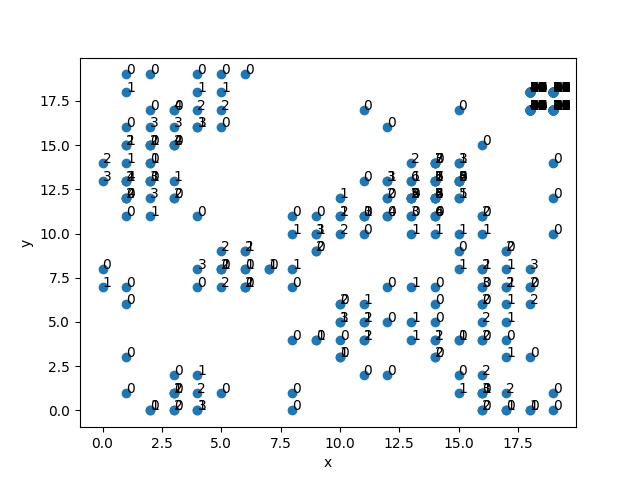
\includegraphics[scale=0.8]{Figure_3.png}
\end{center}
  \caption{Se muestra un mapeo de la matriz.}
  \label{f1}
 
\end{figure}
 
\newpage

\section{Conclusi\'on}

La simulaci\'on del ``juego de la vida'' nos muestra como una matriz se va desarrollando a lo largo de 50 iteraciones en las que existe un declive en el n\'umero de celdas que permanecen activas, ya que, como se mencionaba al principio del experimento, la condici\'on era estar rodeada de otras 3 celdas activas, por lo que, cada iteraci\'on reduci\'a las probabilidades de reunirlas y por lo tanto iban elimin\'andose entre ellas.
En el repositorio\cite{yo} se puede encontrar el archivo en formato gif del comportamiento de la matriz.

\bibliography{tareados}
\bibliographystyle{unsrtnat}


\end{document}